\documentclass{beamer}

% Theme
\usetheme{Copenhagen}
\usecolortheme{dolphin}
\setbeamertemplate{footline}{}
\setbeamertemplate{navigation symbols}{}


% Brazilian Portuguese
\usepackage[brazil]{babel}
\usepackage[utf8]{inputenc}
\usepackage[T1]{fontenc}

% Bibliography
% \usepackage[backend=biber,style=authoryear-icomp]{biblatex}

% Packages
\usepackage{graphicx} % Enables adding figures
\usepackage{subcaption} % Enables figures side-by-side
\usepackage{booktabs} % Makes nicer tables
\usepackage{geometry} % Let's you adjust the margins
\usepackage{setspace} % Let's you change the line spacing
\usepackage{hyperref} % Let's you add links (\url{<link>}) and clickable labels to naviguate through the document
\usepackage{microtype} % Improves the typesetting of your document by managing better the space between letters, hyphens etc.
\usepackage{parskip} % Improves the spacing between paragraphs
\usepackage{amsfonts} % Adds some math fonts

% Shortcuts
\newcommand{\R}{\mathbb{R}} % Shortcut for the set of real numbers
\newcommand{\eps}{\varepsilon} % Shortcut for the epsilon symbol

% Info
\author{Juan Belieni}
\title{Apresentação: implementando o algoritmo de \textit{fuzzy c-means} em Python}
\date{\today}

% Document
\begin{document}

\frame{\titlepage}

\begin{frame}
\frametitle{Introdução}

Como podemos classificar o crescimento econômico de diversos países e identificar padrões de desenvolvimento?

\end{frame}

\begin{frame}
\frametitle{Introdução}
Como podemos classificar o crescimento econômico de diversos países e identificar padrões de desenvolvimento?
\textbf{Clusterização}!
\end{frame}

\begin{frame}
\frametitle{Artigo}
\center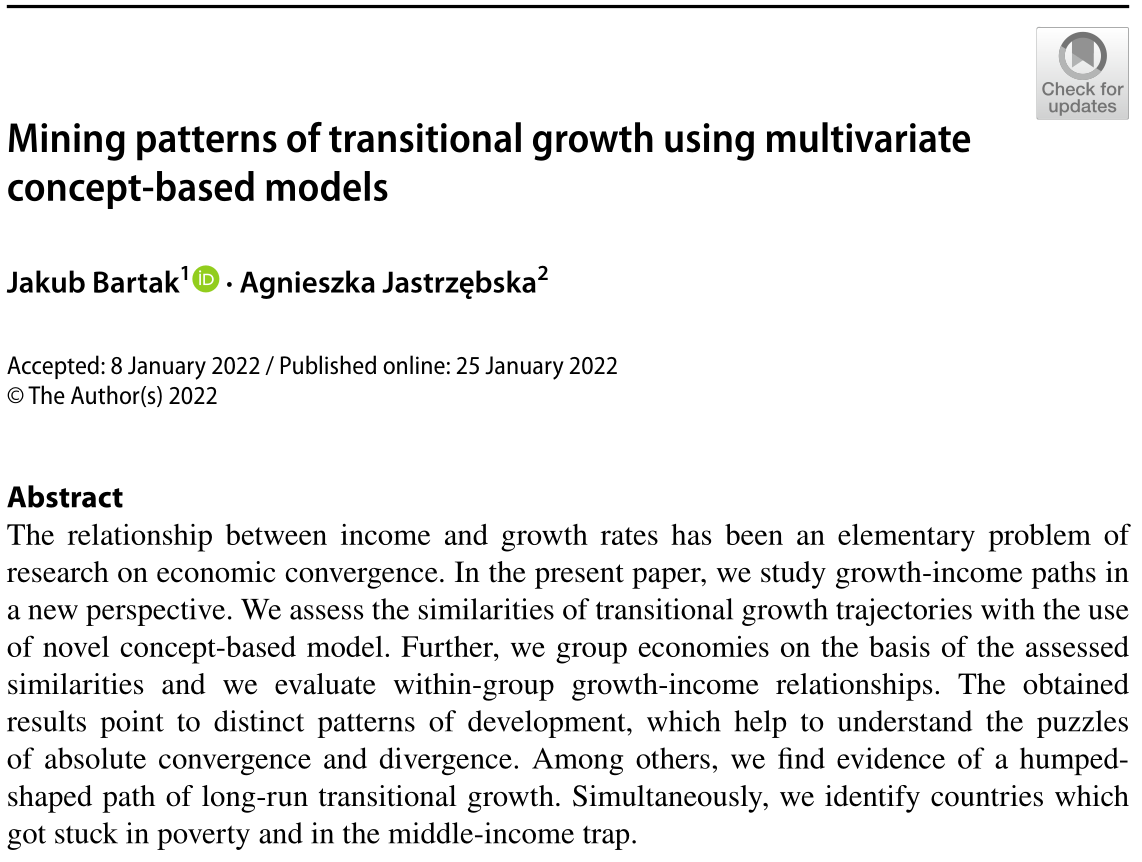
\includegraphics[width=0.75\textwidth]{article.png}
\end{frame}

\begin{frame}
\frametitle{Algoritmo de \textit{fuzzy c-means}}
O algoritmo de \textit{fuzzy c-means} é um algoritmo de clusterização que permite que os pontos pertençam a mais de um cluster.

Mais especificamente, o algoritmo gera uma matriz $U$ que representa o grau de pertencimento de um determinado ponto a cada cluster.

Também é gerado um vetor $\mathbf{v}$ com os centróides de cada cluster.
\end{frame}

\begin{frame}
\frametitle{Função objetivo}
\begin{equation}
J = \sum_{i=1}^P \sum_{j=1}^C u_{ij}^m \| \mathbf z_i - \mathbf v_j \|^2,
\end{equation}

onde

\begin{itemize}
\item $P$ é o número de pontos;
\item $C$ é o número de clusters;
\item $m$ é o coeficiente de fuzzificação.
\end{itemize}
\end{frame}

\begin{frame}
\frametitle{Minimização da função objetivo}

A minimização da função objetivo é feita através da atualização dos graus de pertencimento e dos centróides:

\begin{equation}
u_{ij} = \frac{1}{\sum_{k=1}^C \left( \frac{\| \mathbf z_i - \mathbf v_j \|}{\| \mathbf z_i - \mathbf v_k \|} \right)^{\frac{2}{m-1}}},
\end{equation}

e

\begin{equation}
  \mathbf v_j = \frac{\sum_{i=1}^P u_{ij}^m \mathbf z_i}{\sum_{i=1}^P u_{ij}^m}.
  \end{equation}
\end{frame}

\begin{frame}
\frametitle{Clusterização dos dados de crescimento econômico e PIB per capita}
\center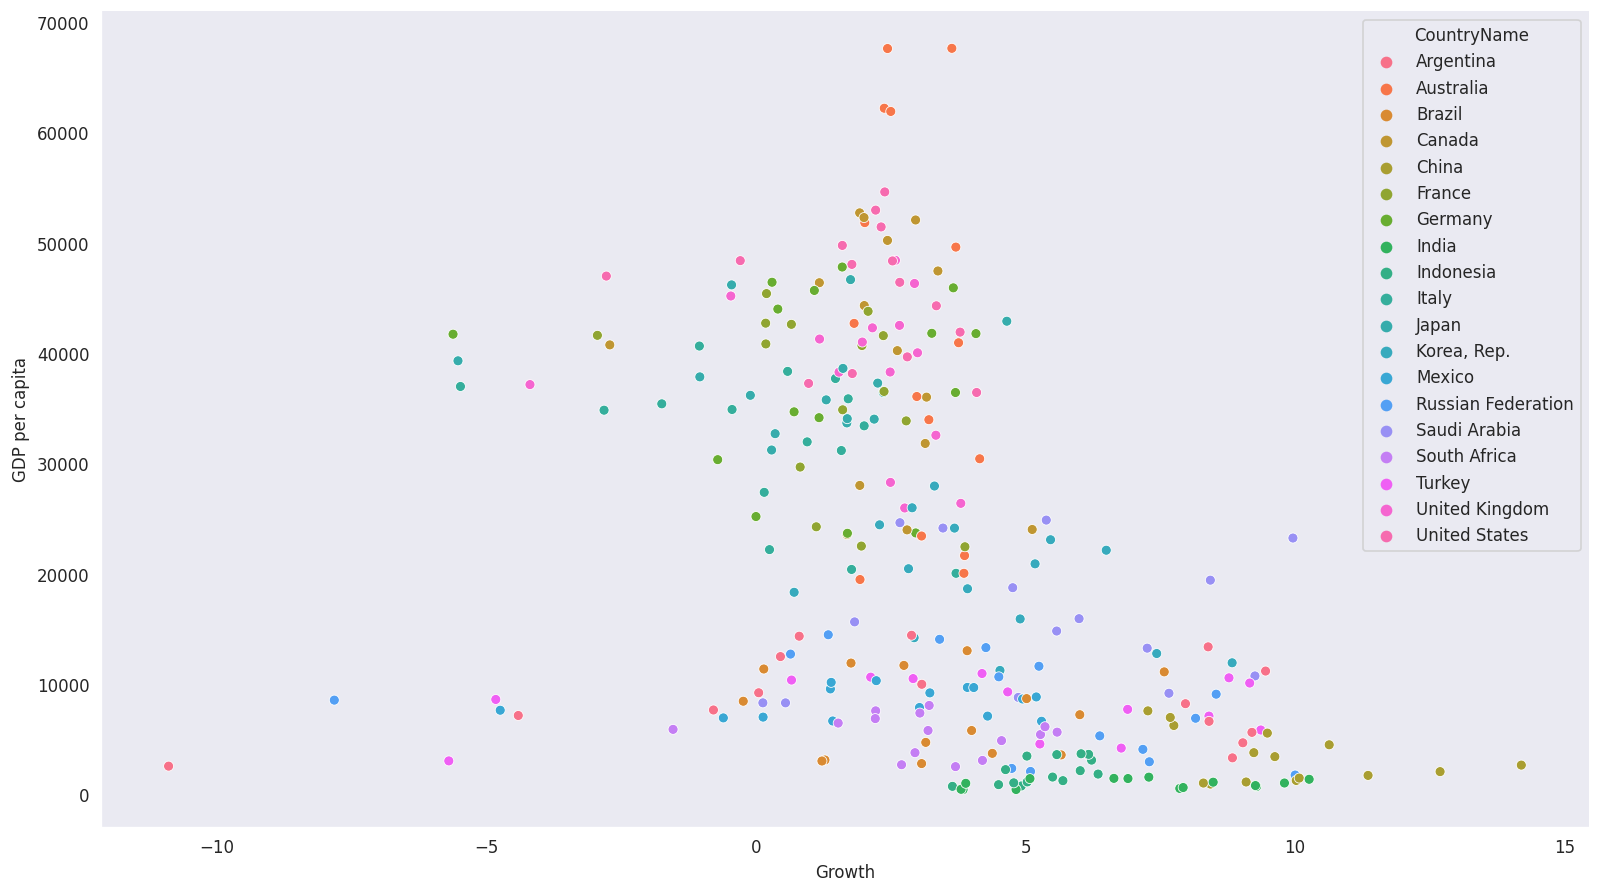
\includegraphics[width=\textwidth]{scatter.png}
\end{frame}

\begin{frame}
\frametitle{Clusterização dos dados de crescimento econômico e PIB per capita}
\center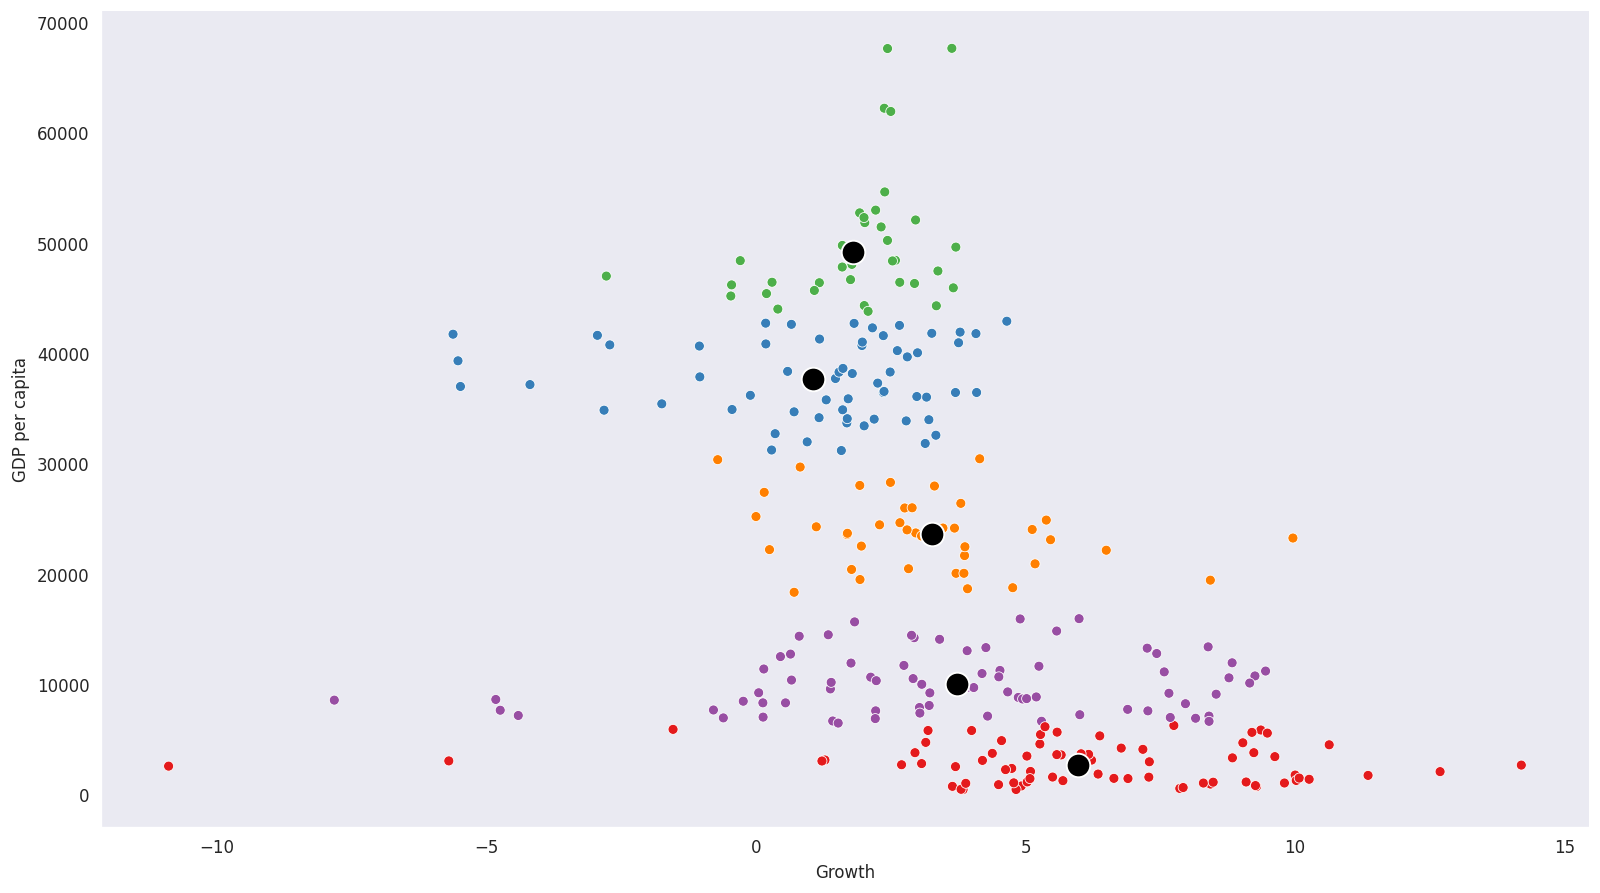
\includegraphics[width=\textwidth]{scatter-cluster.png}
\end{frame}

\begin{frame}
\frametitle{Dendrograma: crescimento econômico e PIB per capita}
\center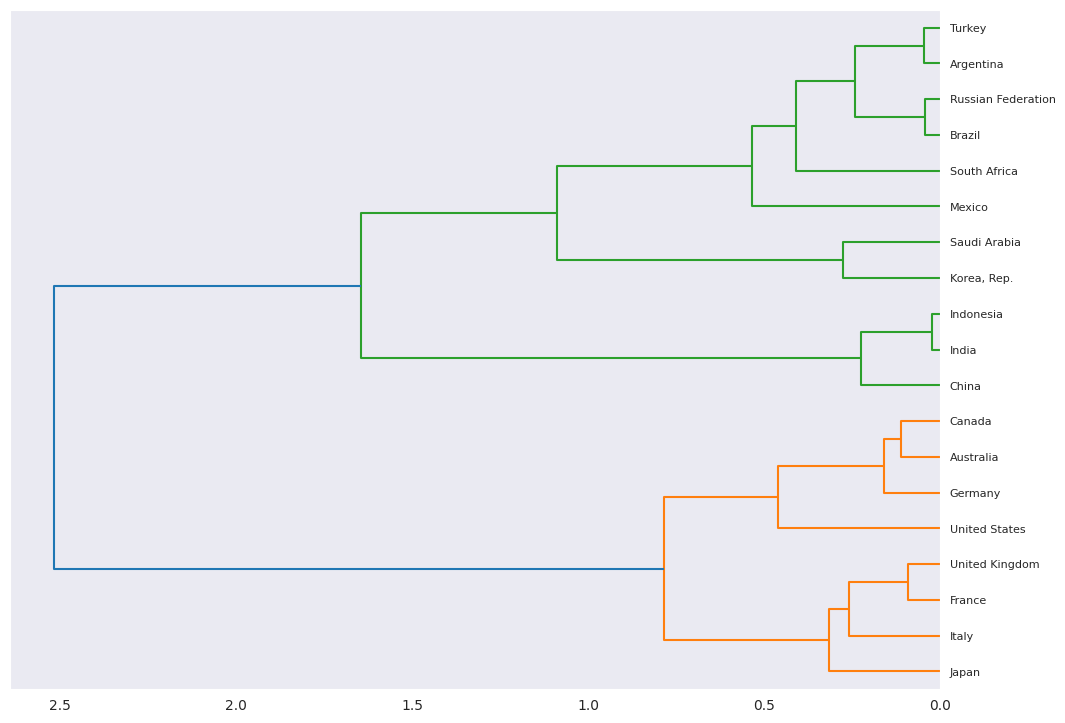
\includegraphics[width=\textwidth]{dendrogram-economy-1.png}
\end{frame}

\begin{frame}
\frametitle{Dendrograma: vários indicadores econômicos}
\small PIB per capita, crescimento econômico, inflação, desemprego e crescimento populacional.
\center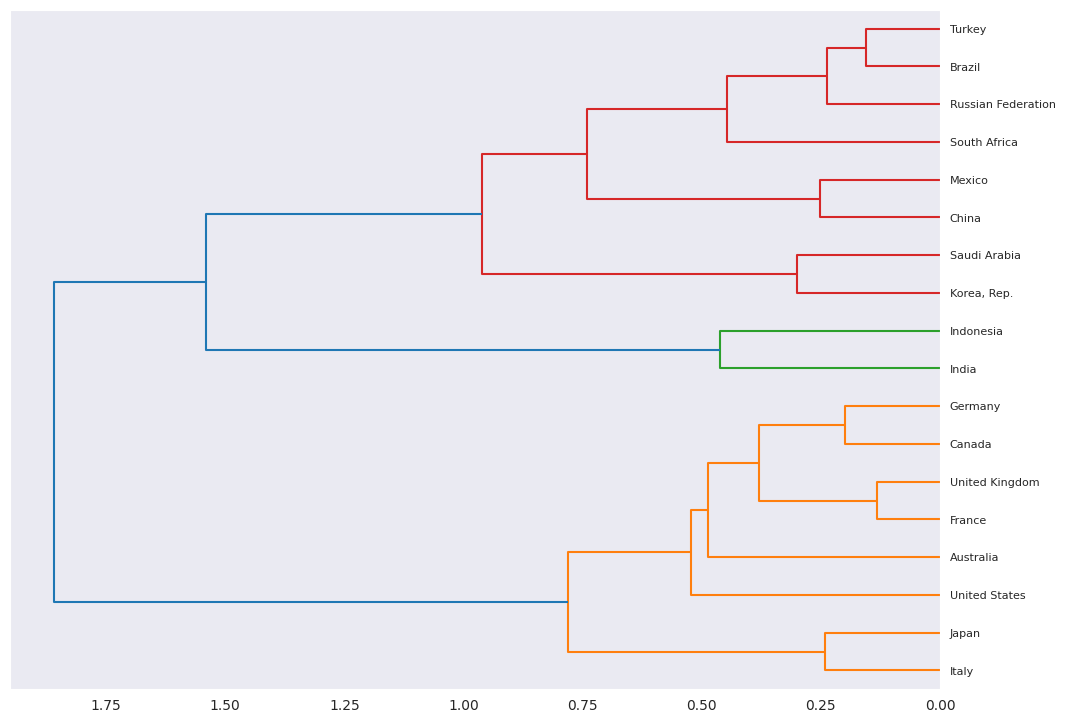
\includegraphics[width=\textwidth]{dendrogram-economy-2.png}
\end{frame}

\end{document}
